\chapter{Risultati}
In questo capitolo si presentano i risultati della fase sperimentale effettuata su tutti i sistemi mostrati precedentemente: classificatore \textit{random forest}, classificatore neurale, autoencoder e GAN. Le metriche di valutazione utilizzate sono enunciate all'interno della sezione \ref{metriche}.

\section{Metriche di valutazione}
\label{metriche}
Le metriche di valutazione utilizzate per testare la qualità dei modelli sono state:
\begin{itemize}
\item \textbf{Precision}: il rapporto $\frac{t_p}{t_p+f_p}$ dove $t_p$ è il numero di veri positivi e $f_p$ il numero di falsi positivi. Intuitivamente è l'abilità del classificatore di non marcare come positivo un campione negativo.
\item \textbf{Recall}: il rapporto $\frac{t_p}{t_p+f_n}$  dove $f_n$ sono i falsi negativi. Intuitivamente è l'abilità del classificatore di trovare tutti i campioni positivi.
\item \textbf{F-score}: è definito come la media armonica tra \textit{precision} e \textit{recall}: 
\[F_1 = 2 \cdot \frac{1}{\tfrac{1}{\mathrm{recall}} + \tfrac{1}{\mathrm{precision}}} = 2 \cdot \frac{\mathrm{precision} \cdot \mathrm{recall}}{\mathrm{precision} + \mathrm{recall}}\]
\item \textbf{Area sottesa da Receiver Operating Characteristic}:  metodo grafico per la valutazione della qualità di un classificatore binario al variare della soglia di discriminazione. E' creata graficando la frazione dei veri positivi rispetto ai campioni positivi ($tpr$ = True positive rate) contro la frazione dei falsi positivi rispetto ai campioni negativi ($fpr$ = False positive rate). L'area sottesa dalla curva ROC equivale alla probabilità che il classificatore predica un campione positivo casuale rispetto ad un campione negativo casuale. Formalmente è definita da:
\[ A = \int_{\infty}^{-\infty} \mbox{TPR}(T) \left(-\mbox{FPR}'(T)\right) \, dT = \int_{-\infty}^{\infty} \int_{-\infty}^{\infty} I(T'>T)f_1(T') f_0(T) \, dT' \, dT = P(X_1 > X_0)\]
dove 
$X_{1}$ è il punteggio per un'istanza positiva e $X_{0}$ è il punteggio per un'istanza negativa, mentre $f_{0}$ e $f_{1}$ sono densità di probabilità che un campione sia negativo ($1$) o positivo ($0$)
\end{itemize}

\section{Classificatore Random Forest}
\label{res:crf}
Il classificatore Random Forest è stato testato in diverse configurazioni. La configurazione che è stata presentata nella sezione \ref{imp:randomforest} ha mostrato i migliori risultati in ogni test.

Il classificatore è stato testato dapprima testato con le seguenti famiglie di malware, contro un subset di dimensione simile di domini provenienti dalla classifica Alexa.

\begin{table}[!htbp]
    \centering
    \begin{tabular}[t]{l}
    \toprule
    Malware Families \\
    \midrule
legit \\
cryptolocker \\
zeus \\
pushdo \\
rovnix \\
tinba \\
conficker \\
matsnu \\
ramdo \\
\bottomrule
\end{tabular}
\caption{\label{tab:malware}}
\end{table}

Il dataset così riunito è stato separato in due parti disuguali: il 90\% è stato utilizzato come dataset di training mentre il restante 10\% come testing in maniera da evitare il fenomeno di overfitting. I risultati della predizione sul dataset di testing sono mostrati di seguito in figura \ref{fig:repdga} e figura \ref{fig:rocdga}. A fianco dell'etichette \textit{legit} e \textit{DGA} è indicato il numero di campioni utilizzati per le due categorie. Come si può notare la performance del classificatore è molto positiva. Si ipotizza che tale risultato sia dovuto alla forte differenza linguistica tra domini reali e domini DGA. 

\begin{figure}[!htbp]
    \centering
    \includegraphics[width=.85\columnwidth]{figures/rndf_tra_nosup_nosup/class_rep.png}
    \caption{Classificatore Random Forest: Report di classificazione su un subset di domini reali (legit) e malevoli (DGA).\label{fig:repdga}}

    \centering
    \includegraphics[width=.85\columnwidth]{figures/rndf_tra_nosup_nosup/roc_plot.png}
    \caption{Classificatore Random Forest: Area sottesa dalla curva ROC per il test con domini di tabella \ref{tab:malware}.\label{fig:rocdga}}
\end{figure}

In fase preliminare si è effettuato un confronto con altri due algoritmi di classificazione: SVC (C-Support Vector) e Gaussian Naive Bayes. La loro performance non è stata altrettanto eccellente e pertanto si è deciso di accantonarli e proseguire con l'utilizzo di Random Forest. I report di classificazione sono mostrati in figura \ref{fig:repsvc} e \ref{fig:repgnb}.

\begin{figure}[!htbp]
  	\centering
    \includegraphics[width=.85\columnwidth]{figures/report_SVC.png}
    \caption{Report di classificazione di SVC.\label{fig:repsvc}}

	\centering
    \includegraphics[width=.85\columnwidth]{figures/report_GaussianNB.png}
    \caption{Report di classificazione di Gaussian Naive Bayes.\label{fig:repgnb}}
\end{figure}

Lo stesso classificatore è stato testato inserendo \textit{suppobox} all'interno delle famiglie DGA. Si è scelto tale malware come campione esterno in quanto presentava la maggiore differenza rispetto alle famiglie mostrate in tabella \ref{tab:malware}. Non è stato fatto un ulteriore training con suppobox. I risultati si possono vedere in figura \ref{fig:repsup} e \ref{fig:rocsup}. Come si può notare la performance ne è fortemente influenzata, introducendo una grande percentuale di falsi nelle predizioni effettuate dal classificatore.

\begin{figure}[!htbp]
    \centering
    \includegraphics[width=.85\columnwidth]{figures/rndf_tra_nosup_sup/class_rep.png}
    \caption{Classificatore Random Forest: Report di classificazione su un subset di domini reali (legit) e malware, comprendenti suppobox (DGA).\label{fig:repsup}}

    \centering
    \includegraphics[width=.85\columnwidth]{figures/rndf_tra_nosup_sup/roc_plot.png}
    \caption{Classificatore Random Forest: Area sottesa dalla curva ROC per il test con  suppobox.\label{fig:rocsup}}
\end{figure}

Come ultimo test è stato eseguito il training aggiungendo al precedente dataset di training una parte di domini generati da suppobox (Figura \ref{fig:repall} e \ref{fig:rocall}). Come si può notare la performance è migliorata sensibilmente, non raggiungendo comunque i risultati eccellenti del primo test.

\begin{figure}[!htbp]
    \centering
    \includegraphics[width=.85\columnwidth]{figures/rndf_tra_sup_sup/class_rep.png}
    \caption{Classificatore Random Forest: Report di classificazione su un subset di domini reali (legit) e malware, comprendenti suppobox (DGA).\label{fig:repall}}

    \centering
    \includegraphics[width=.85\columnwidth]{figures/rndf_tra_sup_sup/roc_plot.png}
    \caption{Classificatore Random Forest: Area sottesa dalla curva ROC per il test con domini reali e malware (comprendenti suppobox).\label{fig:rocall}}
\end{figure}

\section{Classificatore Neurale}
Il classificatore neurale, nato per superare le mancanze del classificatore random forest, è stato testato nelle stesse condizioni utilizzate precedentemente: in particolare è stato utilizzato lo stesso dataset mostrato in sezione \ref{res:crf} e diviso ancora una volta in $\frac{9}{10}$ per la fase di training e $\frac{1}{10}$ per la fase di testing.

Particolarmente difficoltoso si è dimostrato il tuning dei parametri numero epoche e dimensione dei mini-batch per ottenere valori ottimali. Dopo una serie di test sperimentali che hanno messo a confronto diversi valori, si sono rilevati i valori
\begin{itemize}
\item \textbf{numero epoche} $= 60$
\item \textbf{dimensione minibatch} $= 35$ 
\end{itemize}

Tali valori hanno dimostrato di fornire la migliore performance durante la fase di training.

I test effettuati sul dataset, comprendenti suppobox, hanno mostrato i risultati mostrati in figura \ref{fig:cnrepall} e \ref{fig:cnrocall}. Come si può vedere dai grafici il comportamento del classificatore è pressoché identico a quello mostrato dal classificatore random forest (figure \ref{fig:repall} e \ref{fig:rocall} )

\begin{figure}[!htbp]
    \centering
    \includegraphics[width=.85\columnwidth]{figures/clas_nn/class_rep.png}
    \caption{Classificatore Neurale: Report di classificazione su un subset di domini reali (legit) e malware, comprendenti suppobox (DGA).\label{fig:cnrepall}}

    \centering
    \includegraphics[width=.85\columnwidth]{figures/clas_nn/roc_plot.png}
    \caption{Classificatore Neurale: Area sottesa dalla curva ROC per il test con domini reali e malware (comprendenti suppobox).\label{fig:cnrocall}}
\end{figure}

A partire da questo classificatore neurale stabile è stato possibile implementare un sistema di adversarial learning tramite la GAN derivante da un autoencoder. 

\section{Autoencoder}
L'autoencoder come presentato in sezione \ref{autoencoder} è stato testato con il dataset mostrato in sezione \ref{imp:autoencoder:dataset}. In fase sperimentale si è proceduto alla quantificazione della configurazione ottimale dell'autoencoder. In particolare si sono messi a confronto i valori di dropout presenti all'interno di encoder e decoder ed i valori di learning rate.

Di seguito è possibile vedere i risultati della fase di training, per cui si è tenuto $\frac{1}{3}$ del training set come validazione. Come è possibile notare l'ultima iterazione (colore verde) è stata quella che ha mostrato i risultati migliori ed utilizzata come base di partenza per il training della GAN. (Figure \ref{fig:aut1}, \ref{fig:aut2}, \ref{fig:aut3}, \ref{fig:aut4} ).

\begin{figure}[!htbp]
    \centering
    \includegraphics[width=\columnwidth]{figures/autoenc.png}
    \caption{Grafico di Accuracy per le Fase di training dell'autoencoder. La prima fase è rappresentata dalla curva arancione, la seconda dalla curva fuchsia mentre la terza fase è rappresentata dalla curva di colore verde. Si può notare come la precisione senti valori molto alti sul dataset di training per il terzo modello. \label{fig:aut1}}
    \centering
    \includegraphics[width=\columnwidth]{figures/autoenc2.png}
    \caption{Grafico di Loss per la fase di training dell'autoencoder. La prima fase è rappresentata dalla curva arancione, la seconda dalla curva fuchsia mentre la terza fase è rappresentata dalla curva di colore verde. Si può notare come la terza iterazione raggiunge valori accettabilidi loss per il dataset di training.\label{fig:aut2}}
    
\end{figure}
\begin{figure}[!htbp]
    \centering
    \includegraphics[width=\columnwidth]{figures/autoenc3.png}
    \caption{Grafico di accuracy sul dataset di validation per la fase di training dell'autoencoder. Si può notare come i valori raggiunti siano molto simili a quelli ottenuti sul dataset di training.\label{fig:aut3}}   
    \centering
    \includegraphics[width=\columnwidth]{figures/autoenc4.png}
    \caption{Grafico di loss sul dataset di validation per la fase di training dell'autoencoder. Si può notare come i valori raggiunti siano molto simili a quelli ottenuti sul dataset di training.\label{fig:aut4}}
    
\end{figure}
\section{Generative Adversarial Network}
Lorem ipsum dolor sit amet, consectetur adipiscing elit. Etiam ac lorem sed turpis molestie lacinia in a est. Etiam elementum, dolor volutpat varius tristique, est ipsum ornare arcu, hendrerit sagittis mi arcu in turpis. Integer in erat laoreet, facilisis nibh nec, facilisis mauris. Fusce id elit turpis. Donec vestibulum ipsum ac eros gravida pharetra. Integer massa dolor, aliquam a mauris in, mollis molestie mauris. Phasellus varius commodo arcu, in faucibus lorem cursus id. Ut mollis tincidunt ipsum eget viverra. Nullam eget laoreet erat, a venenatis purus. Nunc ut nulla iaculis, faucibus dolor sit amet, tristique purus. Proin feugiat eros sit amet tortor fringilla, quis dapibus libero iaculis. Donec vulputate rhoncus imperdiet. Curabitur ac risus ultricies, feugiat ipsum ut, bibendum lorem. Duis nec convallis tortor. Etiam felis leo, congue vitae odio non, pharetra tristique nisi.

Curabitur eu sapien non tortor tristique feugiat id non justo. Vestibulum in efficitur orci. Nam auctor hendrerit neque sed facilisis. Praesent luctus lorem at mi mattis, vel dapibus turpis fermentum. Quisque eu neque ligula. Suspendisse tincidunt eget quam eget fringilla. Suspendisse et tortor sit amet tortor pulvinar semper. Suspendisse gravida ligula tortor. Donec consequat et sapien at eleifend.

Morbi auctor nunc ultricies risus rutrum, vel tincidunt enim scelerisque. Pellentesque vel leo vitae ligula pellentesque ullamcorper eu in purus. Quisque lorem libero, fringilla at porttitor vel, fringilla vitae urna. Aliquam erat volutpat. Aliquam sit amet tincidunt lacus. Interdum et malesuada fames ac ante ipsum primis in faucibus. Vestibulum iaculis facilisis consectetur. Pellentesque sagittis lorem ut varius finibus. Phasellus ornare efficitur ante non pretium.

Etiam dapibus eleifend turpis, vel dictum nibh rutrum eget. Pellentesque nisi ante, lobortis a ex quis, tristique consequat ex. Nam at sodales mauris, eu ultricies diam. Morbi lobortis urna vel aliquet pulvinar. Proin eu congue nibh. Cras ac metus nec mi volutpat pretium. Duis quis scelerisque enim.

Donec quis egestas nulla. Nullam maximus nulla at nisi laoreet euismod ut id nisi. Nullam fringilla lacus et dui volutpat, ac euismod dui fermentum. Sed tincidunt, neque ornare sollicitudin semper, augue arcu vulputate lectus, sed iaculis lectus lacus in elit. Quisque eleifend mauris id dapibus luctus. Praesent rutrum hendrerit nisi, in placerat purus congue finibus. Nunc pharetra nisl tellus. Fusce nisl leo, vestibulum eu aliquet et, pretium sit amet lorem. Fusce finibus, sapien quis congue blandit, quam diam interdum dui, eu efficitur metus nibh id augue. Pellentesque habitant morbi tristique senectus et netus et malesuada fames ac turpis egestas. Proin aliquet pretium libero eget dignissim. Suspendisse volutpat nunc velit, at fermentum neque blandit ut.
